\section{Heterogeneous Networks and the Need for a Gateway and Bridge}
Consider the typical hourglass network stack in IP-based networks as shown in left-hand image of Figure \ref{fig:hourglass}. This layered design with a thin-waist infrastructure (IP packets for traffic flow) is what enabled the Internet to grow and expand at such a rapid rate; higher layers in the protocol stack extend this communication medium with support for a variety of applications and networking features (e.g., reliable message traversal via TCP). While the NDN architecture introduces a fundamental paradigm shift in the way information is published and retrieved on a network, its design, shown at a high level in the right-hand image of Figure \ref{fig:hourglass}, borrows the same hourglass design as IP networks. Observe that upper layers of the network stack still promote the development of robust applications based on the underlying communication layers. The difference, however, is that network traffic flow management (i.e., to enable reliable and stable communication) and security are \emph{built into} the network stack. These architectural differences mean that application, transport, and network layer protocol semantics in IP-based networks are distinct from protocol semantics in NDN networks. The NDN gateway is intended to bridge between IP and NDN networks by performing this semantic translation between protocols. 

\begin{figure}[ht!]
\begin{center}
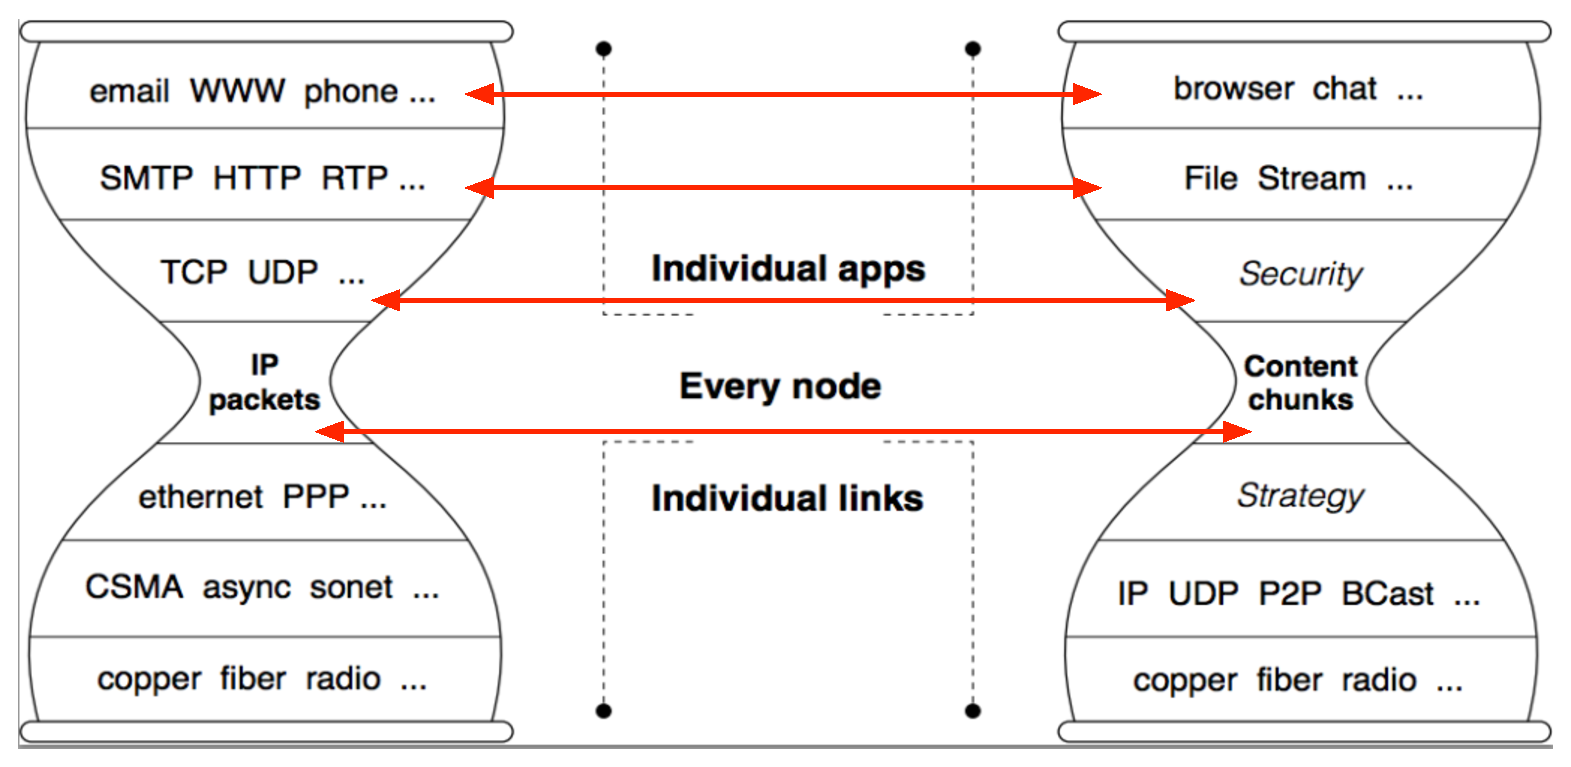
\includegraphics[scale=0.32]{./images/hourglass_conn.pdf}
\label{fig:hourglass}
\caption{A visual comparison of the network stacks for the IP and NDN network architectures.}
\end{center}
\end{figure}

Assuming that NDN is not to be deployed over IP, but instead as a separate network stack entirely, the need for such a gateway cannot be understated. Consider two instances of an application, $A$ and $B$, that wish to send data back and forth to each other. Application $A$ is running on a host with only an IP interface, and application $B$ is running on a host with only an NDN interface. What does it mean for application $A$ to establish a TCP connection stream with application $B$ and what does it mean for application $B$ to issue an interest to application $A$ when neither application speaks the network language of the other. In order for these two applications to communicate, the semantics of a TCP stream-oriented connection must be translated to a stream of contiguous interests, and vice versa. 

Now consider an alternative scenario in which two ``islands'' of NDN hosts exist in isolation, both of which running the same instance of an application. Let host $H_1$ and $H_2$ be a host in the first and second island, respectively, that wish to retrieve data from one another using interests. Without a network route between the two islands, there would be no way for $H_1$ and $H_2$ to interact with one another. However, if there existed two gateways at the borders of each island, each of which connected to the same IP network, then interests from $H_1$ ($H_2$) could be sent to $H_2$ ($H_1)$ as follows:
\begin{enumerate} 
	\item An interest from $H_1$ is intercepted a gateway $G_1$.
	\item $G_1$ encapsulates the interest in an IP packet sent to gateway $G_2$ adhering to IPsec.
	\item $G_2$ unwraps and re-issues the interest and waits for the content to be retrieved from $H_2$. Upon reception, the content's signature is verified and the content is encapsulated in a signed IPsec packet and sent to $G_1$. 
	\item $G_1$ verifies the signature of the packet, creates and signs a new content object, and sends the content object back downstream to $H_1$.
\end{enumerate}

% The gateway middleware is designed so as to support bi-directional traffic flowing from both types of networks. In what follows we describe how traffic in both directions will be supported internally by the gateway.

% \begin{table}[t]
%     \begin{tabular}{|c||c|c|}
%     \hline
%     ~    & {\bf IP} & {\bf NDN} \\ \hline
%     {\bf HTTP} & ~ & ~ \\ \hline
%     {\bf FTP}  & ~ & ~ \\ \hline
%     {\bf SMTP} & ~ & ~ \\ \hline
%     {\bf DNS}  & ~ & ~ \\ \hline
%     \end{tabular}
% \end{table}

\section{Network Semantic Translations at the Gateway}
Traditional IP-based applications and upcoming NDN-based applications treat both the network and content in significantly different ways. In IP-based settings, application and transport layer mechanisms and protocols leverage the underlying IP network layer to send packets to specific hosts. In contrast, in NDN-based settings, there are no straightforward application or transport layer analogs; the network layer, responsible for the issuance of interests and retrieval of content, is abstracted to authenticated (i.e., digitally signed) content objects or streams of data that are consumed by applications. From this perspective, there is no clear bijection between application and transport layer communication in IP-based settings and content and stream-centric data retrieval in NDN-settings. Therefore, to support the interoperability of these two networking paradigms, we need a mechanism to translate the semantics of IP-based communication to and from NDN-based content retrieval. 

The direction of traffic across the gateway has a strong influence on how this semantic translation is done: IP-to-NDN application and transport layer protocols will be mapped to corresponding NDN-interests, and NDN-to-IP traffic (in the form of interests) will be encoded so as to map to the appropriate IP-based application or transport layer protocol. Stateless protocols such as HTTP greatly simplify the job of the gateway because it need not maintain any state to support communication across both networks. However, stateful protocols, such as TCP, naturally require the gateway to maintain state so as to emulate the behavior of an endpoint or host that implements such protocols. For instance, if an IP-based application wishes to establish a TCP connection with an application running on an NDN network to retrieve data, then the gateway must maintain stateful information needed to transform streams of data retrieved over a TCP socket to (packed) discrete and contiguous interests in the NDN network. In what follows we describe the semantic translation details for application and transport layer stateful and stateless protocols in both directions across the gateway.

% \subsection{IP-to-NDN Transport Layer Semantic Translation}
% TODO

% \subsection{IP-to-NDN Application Layer Semantic Translation}
% TODO

% \subsection{NDN-to-IP Transport Layer Semantic Translation}
% TODO

% \subsection{NDN-to-IP Application Layer Semantic Translation}
% TODO

\section{Bridging Isolated Networks via Message Encapsulation at the Bridge}
TODO